\newpage
\section{Question 4: Distributed Transactions}

\subsection{1}

\subsubsection{Node 1}
Since Transaction 2 wants to get an exclusive lock on \texttt{X} it needs to wait until T1 is finished with reading \texttt{X}.
\begin{figure}[htb!]
	\center
	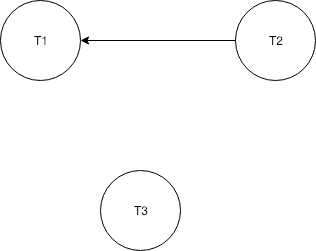
\includegraphics[width=0.5\textwidth]{img/Node1}
	\caption{Waits-for-graph Node 1}
\end{figure}

\subsubsection{Node 2}
Transaction 3 wants to write on \texttt{B} while T2 reads \texttt{B}, so has to wait until T2 is finished.
\begin{figure}[htb!]
	\center
	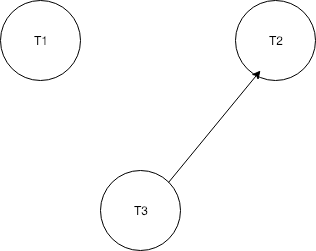
\includegraphics[width=0.5\textwidth]{img/Node2}
	\caption{Waits-for-graph Node 2}
\end{figure}

\subsubsection{Node 3}
Transaction 1 wants to write \texttt{C} and T3 reads \texttt{C}, so T1 has to wait for.
\begin{figure}[htb!]
	\center
	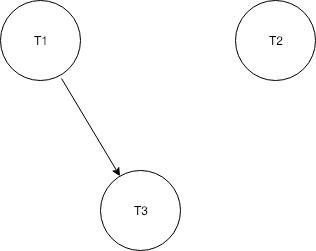
\includegraphics[width=0.5\textwidth]{img/Node3}
	\caption{Waits-for-graph Node 3}
\end{figure}


\subsection{2}
After putting all the wait for graphs together, we get the following global graph.

\begin{figure}[htb!]
	\center
	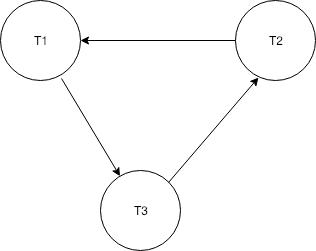
\includegraphics[width=0.5\textwidth]{img/Globalgraph}
	\caption{Global Waits-for-graph}
\end{figure}

\subsection{3}
We don't see any scenario possible where T1 could commit, because we have a deadlock in the global waits for graph so every transaction is waiting on each other.
So in the 2 phase commit protocol the transactions will never reach commit stage and will be aborted.
If we take away T2 or T3 then it would be possible for T1 to commit.
The message exchange would then look like:
\begin{figure}[htb!]
	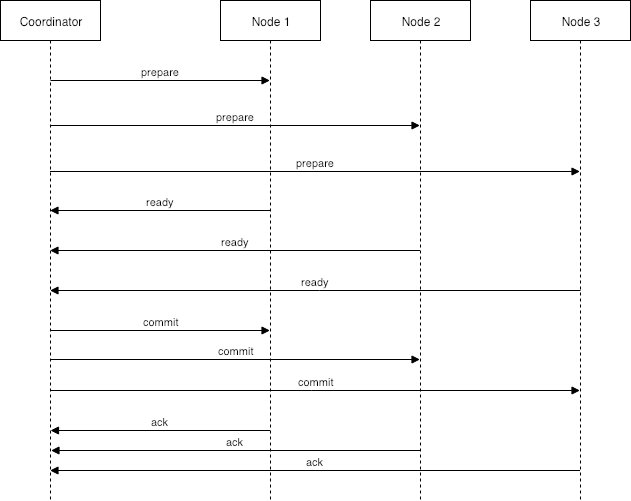
\includegraphics[width=\textwidth]{img/2pcp}
	\caption{2 Phase commit messages}
\end{figure}